\begin{figure*}[t] %!ht
\centering
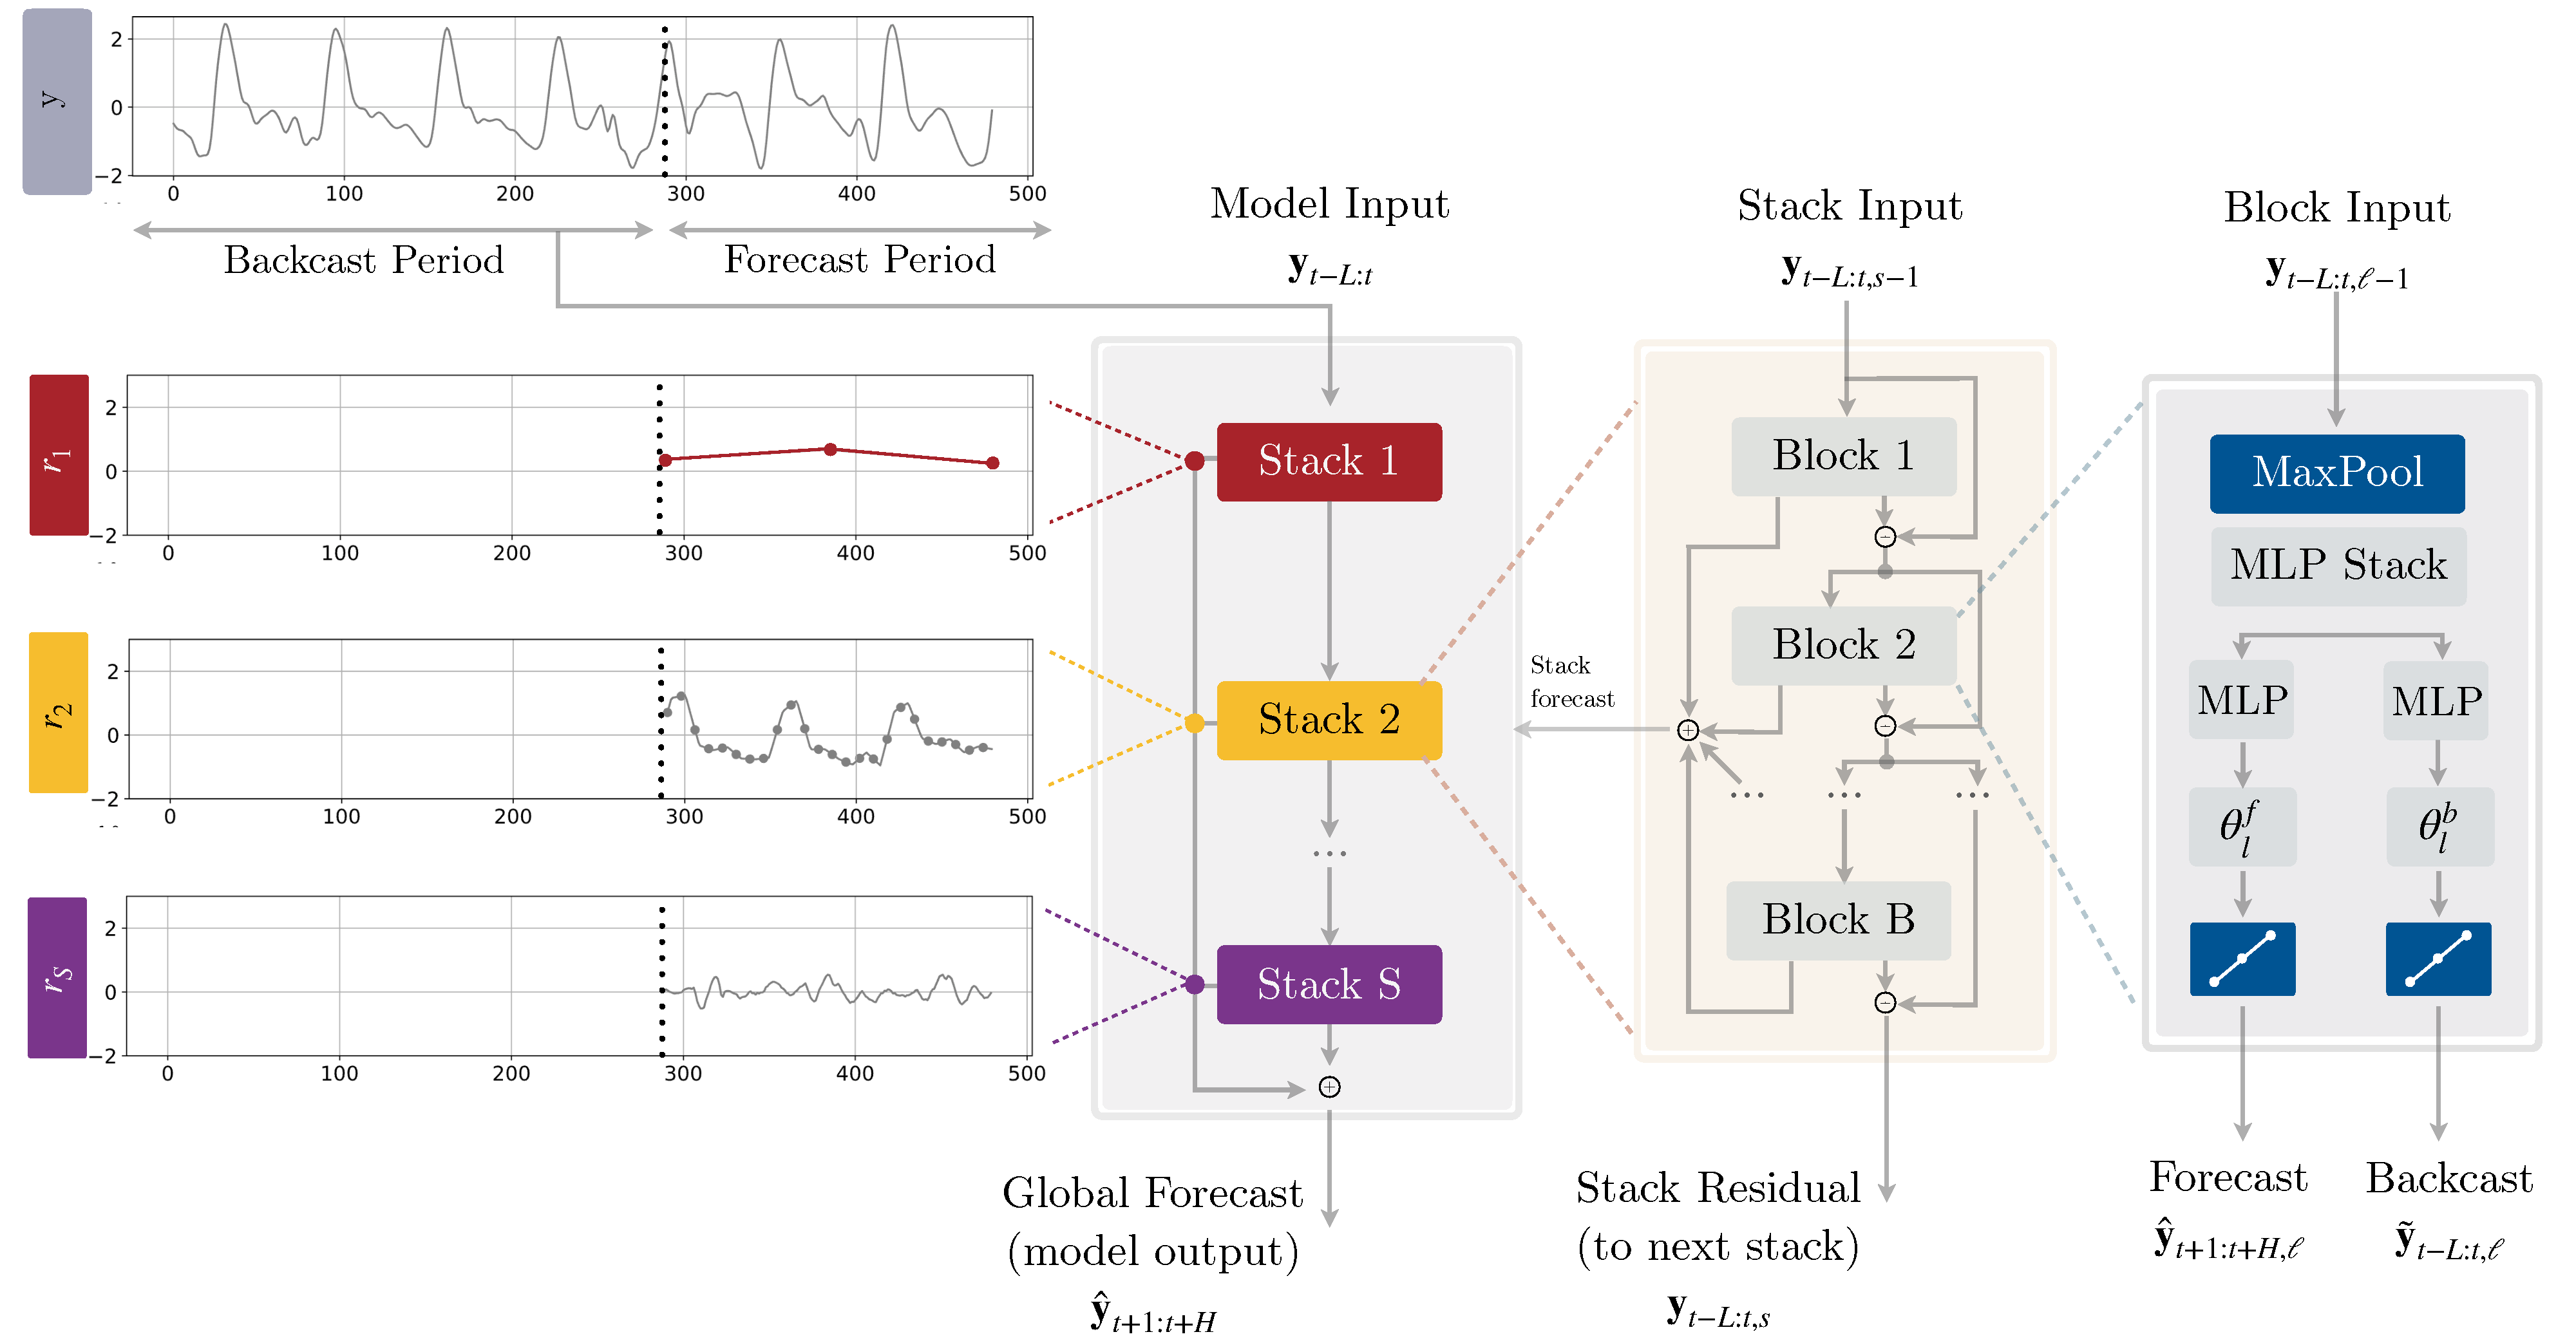
\includegraphics[width=0.9\linewidth]{images/N_HiTS.pdf}
\caption{\ours\  architecture. The model is composed of several MLPs with ReLU nonlinearities. Blocks are connected via doubly residual stacking principle with the backcast $\mathbf{\tilde{y}}_{t-L:t,\ell}$ and forecast $\mathbf{\hat{y}}_{t+1:t+H,\ell}$ outputs of the $\ell$-th block.
Multi-rate input pooling, hierarchical interpolation and backcast residual connections together induce the specialization of the additive predictions in different signal bands, reducing memory footprint and compute time, improving architecture parsimony and accuracy.
}
\label{fig:nhits_architecture}
\end{figure*}

\textbf{Neural forecasting.} Over the past few years, deep forecasting methods have become ubiquitous in industrial forecasting systems, with examples in optimal resource allocation and planning in transportation \citep{laptev2017neural_forecasting_uber}, large e-commerce retail \citep{wen2017mqrcnn, olivares2021probabilistic_hierarchical_dpm, paria2021hierarchical_hired, rangapuram2021hierarchical_e2e}, or financial trading \citep{banushev_barclay2021neural_forecasting_aws}. The evident success of the methods in recent forecasting competitions \citep{makridakis2020m4_competition, makridakis2021m5_competition} has renovated the interest within the academic community \citep{benidis2020dl_timeseries_review2}. In the context of multi-variate long-horizon forecasting, Transformer-based approaches have dominated the landscape in the recent years, including \Autoformer~\citep{wu2021autoformer}, an encoder-decoder model with decomposition capabilities and an approximation to attention based on Fourier transform, \Informer~\citep{zhou2021informer}, Transformer with MLP based multi-step prediction strategy, that approximates self-attention with sparsity, \Reformer~\citep{kitaev2020reformer}, Transformer that approximates attention with locality-sensitive hashing and \LogTrans~\citep{li2019logtrans}, Transformer with local/log-sparse attention.

\textbf{Multi-step forecasting.} Investigations of the bias/variance trade-off in multi-step forecasting strategies reveal that the \emph{direct} strategy, which allocates a different model for each step, has low bias and high variance, avoiding error accumulation across steps, exhibited by the classical \emph{recursive} strategy, but losing in terms of net model parsimony. Conversely, in the \emph{joint} forecasting strategy, a single model produces forecasts for all steps in one shot, striking the perfect balance between variance and bias, avoiding error accumulation and leveraging shared model parameters~\citep{bao2014msvr, atiya2016multi_step_forecasting, wen2017mqrcnn}. 

\textbf{Multi-rate input sampling.} Previous forecasting literature recognized challenges of extremely long horizon predictions, and proposed \emph{mixed data sampling regression} (\MIDAS; \citealt{ghysels2007midas_regressions, armesto2010ForecastingWMF}) to ameliorate the problem of parameter proliferation while preserving high frequency temporal information. \MIDAS\ regressions maintained the classic \emph{recursive} forecasting strategy of linear auto-regressive models, but defined a parsimonious fashion of feeding the inputs. 

\textbf{Interpolation.} Interpolation has been extensively used to augment the resolution of modeled signals in many fields such as signal and image processing~\citep{meijering2002interpolation_history}. In time-series forecasting, its applications range from completing unevenly sampled data and noise filters \cite{chow1971interpolation_extrapolation_time_series, roque1981interpolation_time_series_note, shukla2019interpolation_prediction_networks, rubanova2019latent_odes_irregular_sample} to fine-grained quantile-regressions with recurrent networks \citep{gasthaus2019spline_quantile_function}. To our knowledge, temporal interpolation has not been used to induce multi-scale hierarchical time-series forecasts.
